\chapter{Расчет излучения источников}\label{radiation}
FAINA позволяет рассчитывать электромагнитное излучение от источников с заданными функциями распределения излучающих частиц и другими параметрами. Построены модели следующих типов излучения: синхротронного, обратного комптоновского рассеяния, пионного распада в результате свободно-свободного взаимодействия протонов и тормозного излучения.
\section{Функции распределения частиц}
Важнейшими исходными данными для расчета любого типа излучения является функция распределения излучающих частиц. В коде FAINA для представления распределений используется абстрактный класс ParticleDistribution и семейство наседованных от него классов, соответствующих различным конкретным реализациям. Класс ParticleDistribution имеет следующие доступные методы, описанные в Таблице \ref{ParticleDistribution}:
	\begin{table}
	\begin{center}
		\begin{small}
		\begin{tabularx}{\textwidth}{|X|X|}
			\hline
			\textbf{ParticleDistribution} & \\
			\hline
			distribution(const double\& energy, const double\& mu, const double\& phi) & возвращает функцию распределения от энергии, косинуса полярного угла и азимутального угла, нормированную на единицу \\
			\hline
			distributionNormalized(const double\& energy, const double\& mu, const double\& phi) & возвращает функцию распределения от энергии, косинуса полярного угла и азимутального угла, нормированную на концентрацию \\
			\hline
			getConcentration() & возвращает концентрацию частиц\\
			\hline
		\end{tabularx}
	    \end{small}
    	\caption{Публичные методы класса ParticleDistribution }
    	\label{ParticleDistribution}
	\end{center}
\end{table}

Для вычисления излучения необходимо в первую очередь задать распределение излучающих частиц. Для это нужно создать объект из подходящего класса-наследника ParticleDistribution. Дерево наследования на две большие ветви - распределения фотонов, представленных абстрактным классом PhotonDistribution и распределения массивных частиц - MassiveParticleDistribution. Схема наследования этих классов представлена на рисунке \ref{particleDistribution0}. 
\begin{figure}
	\centering
	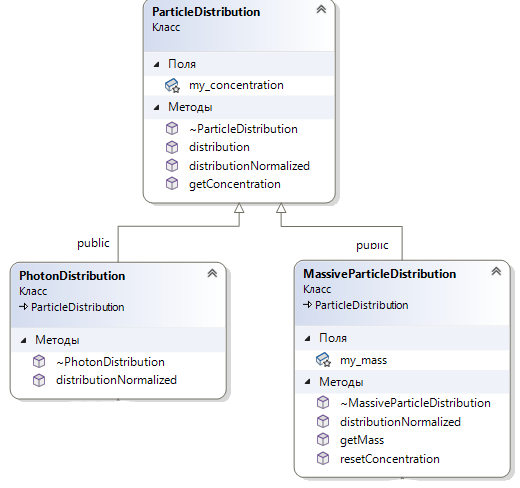
\includegraphics[width=9.5 cm]{./fig/particleDistribution0.png} 
	\caption{Схема наследования распределения фотонов и массивных частиц}
	\label{particleDistribution0}
\end{figure}
Важно отметить, что распределения фотонов не используются для представления результатов расчета излучения. Они нужны как входной параметр для расчета обратного комптоновского рассеяния. Класс PhotonDistribution не имеет дополнительных собственных методов и является лишь интерфейсом. Класс MassiveParticleDistribution тоже является абстрактным, в нем не задан конкретный вид распределения, но добавлены новые методы, описанные в Таблице \ref{MassiveParticleDistribution}	
\begin{table}
	\begin{center}
		\begin{small}
			\begin{tabularx}{\textwidth}{|X|X|}
				\hline
				\textbf{MassiveParticleDistribution} & \\
				\hline
				getMass() & возвращает массу частиц \\
				\hline
				resetConcentration(const double\& n) & позволяет изменить полную концентрацию частиц в распределении\\
				\hline
			\end{tabularx}
		\end{small}
		\caption{Публичные методы класса MassiveParticleDistribution }
		\label{MassiveParticleDistribution}
	\end{center}
\end{table}
\subsection{Распределения фотонов}

От абстрактного класса PhotonDistribution наследуются следующие классы: абстрактный PhotonIsotropicDistribution, предназначенный для представления изотропных распределений фотонов и CompoundPhotonDistribution, представляющий из себя сумму нескольких распределений фотонов общего вида. Схема наследования классов фотонных распределений представлена на рисунке \ref{photonDistribution}.
\begin{figure}
	\centering
	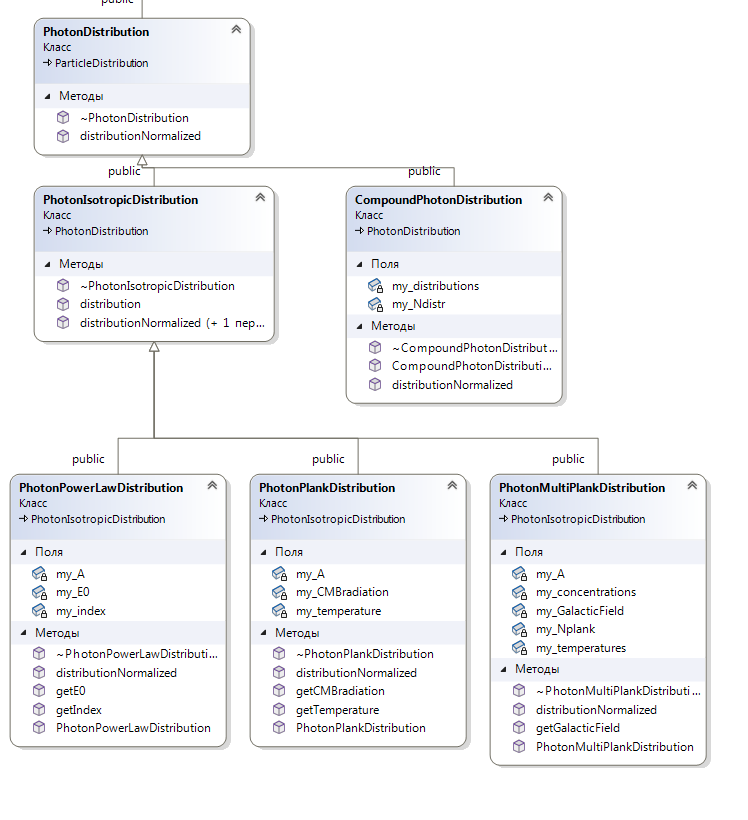
\includegraphics[width=10.5 cm]{./fig/photonDistribution1.png} 
	\caption{Схема наследования распределения фотонов и массивных частиц}
	\label{photonDistribution}
\end{figure}

У изотропного распределения PhotonIsotropicDistribution добавляются методы, возвращающие значение функции распределения только в зависимости от энергии. Важно понимать, что это не функция распределения по энергии, а полная функция распределения с отброшенными угловыми аргументами. Другими словами, для получения значения функции распределения по энергии нужно домножить значение, возвращенное данным методом на $4 \pi$.

У класса PhotonIsotropicDistribution есть три наследника, которые уже не абстрактные классы, а непосредственно предназначены для создания распределений. Это PhotonPowerLawDistribution для представления степенных распределений, PhotonPlankDistribution, для планковских распределений и PhotonMultiPlankDistribution, для суммы планковских распределений. Метода класса PhotonIsotropicDistribution и его наследников перечислены в таблице \ref{photonDistributionMethods}
\begin{table}[h!]
	\begin{center}
		\begin{small}
			\begin{tabularx}{\textwidth}{|X|X|}
				\hline
				\textbf{PhotonIsotropicDistribution} & \\
				\hline
				distribution(const double\& energy) & возвращает функцию распределения с отброшенными угловыми аргументами, то есть нормированную на концентрацию, деленную на $4 \pi$ \\
				\hline
				distributionNormalized(const double\& energy) & возвращает функцию распределения с отброшенными угловыми аргументами, нормированную на  $ 1 / 4 \pi$\\
				\hline
				\textbf{PhotonPowerLawDistribution} & \\
				\hline
				PhotonPowerLawDistribution(const double\& index, const double\& E0, const double\& concentration) & конструктор, создающий экземпляр с заданными показателем наклона, начальной энергией и полной концентрацией \\
				\hline
				getIndex() & возвращает показатель наклона спектра\\
				\hline
				getE0() & возвращает минимальную энергию степенного распределения\\
				\hline
				\textbf{PhotonPlankDistribution} & \\
				\hline
				PhotonPlankDistribution(const double\& temperature, const double\& amplitude) & конструктор, создающий экземпляр с заданными температурой и апмплитудой - то есть отношением концентрации к равновесному планковскому распределению с данной температурой\\
				\hline
				static getCMBRadiation() & статический метод, возвращающий экземпляр, соответствующий реликтовому излучению (температура $2.725 K$, амплитуда $1$)\\
				\hline
				getTemperature() & возвращает температуру распределения\\
				\hline
				\textbf{PhotonMultiPlankDistribution} & \\
				\hline
				PhotonMultiPlankDistribution(int Nplank, const double* const temperatures, const double* const amplitudes) & конструктор, количество планковских распределений, участвующих в смеси, массив их температур и массив амплитуд\\
				\hline
				static getGalacticField() & статический метод, возвращающий экземпляр, соответствующий среднегалактическому фотонному распределению, по данным статьи \cite{Mathis1983} \\
				\hline
			\end{tabularx}
		\end{small}
		\caption{Публичные методы классов изотропных распределений фотонов}
		\label{photonDistributionMethods}
	\end{center}
\end{table}

Класс CompoundPhotonDistribution предназначен для представления смеси различных распределений фотонов, не обязательно планковских, как PhotonMultiPlankDistribution, и не обязательно изотропных. Его методы описаны в Таблице \ref{CompoundPhotonMethods}
\begin{table}[h!]
	\begin{center}
		\begin{small}
			\begin{tabularx}{\textwidth}{|X|X|}
				\hline
				\textbf{CompoundPhotonDistribution} & \\
				\hline
				CompoundPhotonDistribution(int N, PhotonDistribution** distributions) & конструктор, создающий экземпляр с заданным количеством распределений в смеси и массивом этих распределений \\
				\hline
				CompoundPhotonDistribution(PhotonDistribution* dist1, PhotonDistribution* dist2) & конструктор, создающий экземпляр содержащий смесь из двух распределений\\
				\hline
				CompoundPhotonDistribution(PhotonDistribution* dist1, PhotonDistribution* dist2, PhotonDistribution* dist3) & конструкторб создающий экземпляр содержащий смесь из трех распределений\\
				\hline
			\end{tabularx}
		\end{small}
		\caption{Публичные методы класса CompoundPhotonDistribution }
		\label{CompoundPhotonMethods}
	\end{center}
\end{table}

Встроенных анизотропных распределений фотонов в коде на данный момент нет, но пользователь может реализовать их самостоятельно, создав класс, наследующий от PhotonDistribution и определив необходимый виртуальный метод distributionNormalized(const double\& energy, const double\& mu, const double\& phi). Аналогично можно, конечно, создать и другие виды изотропных распределений.

\subsection{Распределения массивных частиц}
Распределения массивных частиц представлены наследниками класса MassiveParticleDistribution